\chapter{General Introduction}
%\addstarredchapter{General Introduction}
%-------------------------------------------------------------------------------------------------------------------------------------------------
\textbf{Macrosegregation} is a very known defect to metallurgical processes. Despite a great evolution achieved by active research during the last 60 years,
it remains partially understood. Macrosegregation is often  the consequence of several factors at the scale of a casting, all related to \emph{microsegregation} happening at the scale
of dendrites. Today, research in metallurgy focuses on a deeper understanding of such a connection between the different physical scales.
Solidification is not only a phase change, but also a complex transformation involving small scales like nucleation, medium scales
like grains growth and large scales like convection in the melt. From the nucleation theory to the mechanical behavior of metals, intricate phenomena combine to form defects in the final product. This has been seen in casting processes, such as continuous casting (\cref{fig:cc_process}) and ingot casting. Surface and volume porosity, hot tearing and composition heterogeneity are known defects to the casting community. After a brief introduction of these defects, macrosegregation will be the focus of this dissertation. 

\begin{figureth}
% textwidth 
{1.0}
%path 
{Chapter0/Graphics/cc_process}
% caption
{Main steps in a continuous casting plant}
% label
\label{fig:cc_process}
\end{figureth}
%-------------------------------------------------------------------------------------------------------------------------------------------------
\section{Casting defects}
Undesired effects are inevitable in any industrial process. More importantly, a lot of defects in the casting industry can be disastrous in some situations where the cast product is not serviceable and hence rejected. This leads to a systematic product recycling, i.e. the product is ditched to be reheated, remelted and then cast again. From an economic point view, the operation is expensive timewise and profitwise. Understanding and preventing defects when possible, is thus crucial in the casting industry. We focus hereafter on the main encountered defects.
%-------------------------------------------------------------------------------------------------------------------------------------------------
\subsection*{Hot tearing} 
This defect, also denoted solidification cracking or hot cracking, occurs in the mushy zone at high solid fractions when a failure
or crack appears at specific locations, the hot spots. The temperature range in which the steel is vulnerable to hot tearing is known as the brittleness temperature range (BTR). It corresponds to solid fractions greater than \num{90}\%, with the liquid phase forming a discontinuous film. Many factors can cause the failure, but the main origin is a lack of liquid feeding required to compensate for the solidification shrinkage, in the presence of thermal stresses in the mushy region. Therefore, a crack initiates then propagates in the casting, as shown in \cref{fig:hottearing}. 
\begin{figureth}
% hottearing1: JM drezet, GDR 2013 Lausanne, contraintes residuelles.
% textwidth 
{0.4}
%path 
{Chapter0/Graphics/hottearing1.png}
% caption
{Crack in an aluminium slab}
% label
\label{fig:hottearing}
\end{figureth}
%-------------------------------------------------------------------------------------------------------------------------------------------------
\subsection*{Porosity}
%reference: \url{http://www.afsinc.org/about/content.cfm?ItemNumber=6933} \\
%reference: \url{http://en.wikipedia.org/wiki/Casting_defect} \\
Porosity is a void defect formed inside the casting or at the outer surface. It may attributed to two different factors.
Firstly, we speak of \emph{shrinkage porosity}, when a void forms as a result of density differences between the interdendritic liquid and solid
network, the latter being denser than the former (\cref{fig:porosity3,fig:porosity4}). It is basically, the same reason that initiates hot cracks. 
The second factor is the presence of dissolved gaseous phases in the melt (\cref{fig:porosity1,fig:porosity2}). According to \citet{dantzig_solidification_2009}, these gases may be initially in the melt, or created by the reaction between the metal and water found in the air or at trapped in grooves at the moulds surface. If the decreasing temperature and pressure drop in the liquid are large enough, the latter becomes supersaturated. Consequently, the nucleation of gaseous phase is triggered (just like when you a cold bottle of coca-cola is opened !).
\begin{figure}[htbp] %h!
%Porosity1-2: http://www.afsinc.org/about/content.cfm?ItemNumber=6933
%Porosity3: http://www.weldreality.com/aluminumalloys.htm
%Porosity4: http://www.esab.com/global/en/education/new-lean-duplex-steels.cfm
\centering
   %------------
  \begin{subfigure}[t]{0.3\textwidth}
    \centering
	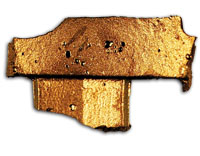
\includegraphics[width=\textwidth]{Chapter0/Graphics/porosity1.jpg}
	\caption{Gas porosity in casting}
    \label{fig:porosity1}
  \end{subfigure}
   %------------
   \hspace{1cm}
   \begin{subfigure}[t]{0.25\textwidth}
    \centering
	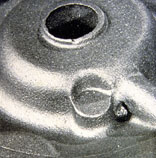
\includegraphics[width=\textwidth]{Chapter0/Graphics/porosity2.jpg}
	\caption{Shrinkage porosity}
    \label{fig:porosity2}
  \end{subfigure}
  %------------------------------
  \vskip\baselineskip
  %------------------------------
  \begin{subfigure}[t]{0.3\textwidth}
    \centering
	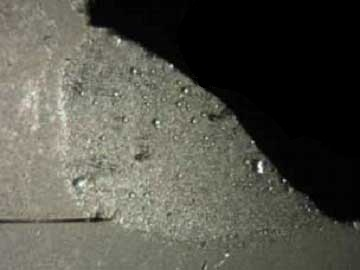
\includegraphics[width=\textwidth]{Chapter0/Graphics/porosity3.jpg}
	\caption{Gas porosity in aluminium welding}
    \label{fig:porosity3}
  \end{subfigure}
   %------------
  \hspace{1cm}
   \begin{subfigure}[t]{0.25\textwidth}
    \centering
	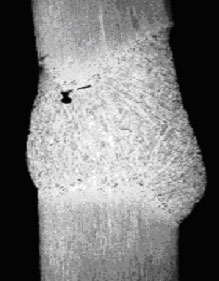
\includegraphics[width=\textwidth]{Chapter0/Graphics/porosity4.jpg}
	\caption{Xray of volume void inside welded duplex steel}
    \label{fig:porosity4}
  \end{subfigure}
   %------------
\caption{Examples of porosity in casting and welding} 
\label{fig:porosity}
\end{figure}
%-------------------------------------------------------------------------------------------------------------------------------------------------
\subsection*{Freckles or segregated channels} 
The origin of this defect is a combined effet of microsegregation and buoyancy forces. 
Upon solidification, solid forms while rejecting some solute in the liquid due to partitioning (steels have a partition coefficient less than unity).
When segregated solute is the lighter species, an increasing concentration in the liquid phase produces a solutal driving force inside the mushy zone, generating unstable convection currents, with "plume" shapes as often reported in the literature \citep{sarazin_studies_1992, schneider_modeling_1997, shevchenko_chimney_2013}. When temperature gradient is an additional force of convection, the latter is hence qualified as "thermosolutal".
%-------------------------------------------------------------------------------------------------------------------------------------------------
\section{Macrosegregation}
Macrosegreation generally stems from a solubility difference between a liquid phase and one or more solid phases, along with
a relative velocity between these phases. While the former is responsible for local solute enrichment or depletion, the latter
will create the composition heterogeneity on a scale much larger than just a few dendrites.
% http://dictionary.cambridge.org/grammar/british-grammar/little-a-little-few-a-few
This is why macrosegregation could be observed on the scale of a casting, up to several meters in length. 
%--------------------------------------------------------
\subsection{Causes}
Four main factors can (simultaneously) cause fluid flow leading to macrosegregation:
\subsubsection*{Liquid dynamics}
During solidification, thermal and solutal gradients result in density gradients in the liquid phase: 
\begin{subequations}
\begin{align}
\label{eq:rholiq}
& \rhol = \rhoref ( 1 - \betaT (T - \Tref) - \sum_{i} \betawil (\wil - \wilref) )  \\ 
\label{eq:gradrholiq}
& \nabvec\rhol = -\rhoref (  \betaT \nabvec T + \sum_{i} \betawil \nabvec\wil  )
\end{align}
\end{subequations}
In \cref{eq:rholiq}, density is assumed to vary linearly with temperature and phase composition for each chemical species (index $i$).
The slopes defining such variations are respectively the thermal expansion coefficient $\betaT$ and solutal expansion coefficient $\betawil$, given by \citep{kohler_peritectic_2008}:
\begin{subequations}
\begin{align}
\label{eq:betaT}
& \betaT =  -\frac{1}{\rhoref} \brac{\frac{\partial\rhol}{\partial T}}  \\ 
\label{eq:betawil}
& \betawil = -\frac{1}{\rhoref} \brac{\frac{\partial \rhol}{\partial \wil}}  
\end{align}
\end{subequations}
The linear fit assumes also that the density takes a reference value, $\rhoref$, when temperature and liquid composition reach reference values, respectively
$\Tref$ and $\wilref$. However, in some situations, a suitable thermodynamic database providing accurate density values is far better than a linear fit, especially in the current context of macrosegregation. 
Such possibility will be discussed later in the manuscript (cf. SECTION TODO ) %TODO 
In the presence of gravity, the density gradient in \cref{eq:gradrholiq}, causes thermosolutal convection in the liquid bulk and a subsequent macrosegregation.
 
\subsubsection*{Solidification shrinkage}
Solid alloys have a greater density than the liquid phase ($\rhos > \rhol$), thus occupy less volume. Upon solidification, the liquid moves towards the solidification front to compensate for the volume difference caused by the phase change, as well as the thermal contraction. When macrosegregation is triggered by solidification shrinkage,
we speak of \emph{inverse segregation} Theoretically, if solute mass is conserved, a decreasing volume results in a positive segregation. Shrinkage deforms the outer
surface of a solidifying alloy, causing positive macrosegregation. While one would naturally expect negative macrosegregation in areas where solidification begins and positive inside the alloy, shrinkage promotes the opposit phenomenon, hence the term \emph{inverse segregation}.
In contrast to liquid convection, shrinkage flow may cause macrosegregation even without gravity.

\subsubsection*{Movement of equiaxed grains}
Equiaxed grains can grow in the liquid bulk where thermal gradients are weak, or in the presence of inoculants. Consequently, 
they are transported by the flow (floating or sedimenting, depending on their density \citep{beckermann_modelling_2002}) which leads to negative macrosegregation in their final position.

\subsubsection{Solid deformation} 
Stresses of thermal and mechanical nature are always found in casting processes (e.g. bulging between rolls in continuous casting). 
Deformation of the semi-solid in the mushy zone causes a relative solid-liquid flow in the inward (tensile stresses) or outward (compression stresses) direction, causing macrosegregation.
%--------------------------------------------------------------------------------------------------------------------------------------------------
\subsection{Types}
\subsubsection*{In continuous casting}
The semi-solid billet is carried through a series of rolls that exert a radial force to straighten it and get it to its horizontal position.
As the mushy part of a slab enters through these rolls, interdendritic liquid is expelled backwards, i.e. regions with lower solid fraction.
Since the the boundaries solidify earlier than the centre, the enriched liquid accumulates halfway in thickness, forming a centreline macrosegregation
as shown in \cref{fig:macroseg_centreline}. Other types of segregates (channels, A-segregates ...) can also be found but remain more specific to ingot casting. 
\begin{figureth}
% macrosegregation_centreline_zoom: http://goo.gl/iKPNfz
% textwidth 
{1.0}
%path 
{Chapter0/Graphics/macrosegregation_centreline_zoom.pdf}
% caption
{Centreline segregation in a steel slab \citep{beckermann_modelling_2002}}
% label
\label{fig:macroseg_centreline}
\end{figureth}
%--------------------------------------------------------
\subsubsection*{In ingot casting}
A variety of segregation patterns can be encountered in heavy ingots: 
\begin{itemize}
\itemsep0em 
\item the lower part is characterized by a negative segregation cone promoted by the sedimentation of 
	  equiaxed crystals,
\item positive segregation channels, known as A-segregates, form along the columnar dendritic zones, close to the vertical contact with the mould,
\item positive V-segregates can be identified in the centre of the ingot,
\item a positive macrosegregation in the upper zone where the last liquid solidifies, the so-called "hot-top", caused by solidification shrinkage (inverse segregation)
	  and thermosolutal buoyancy forces. 
\end{itemize}
\citet{combeau_prediction_2009} state that A-segregates and V-segregates formation is mainly attributed to local flow phenomena.
As such, their scale is finer than macrosegregation, hence called "mesosegregates".
%-----------------------
\begin{figureth}
{0.6}
{Chapter0/Graphics/macrosegregation_ingot.png}
{Sulphur print (left) of a 65-ton steel ingot \citep{lesoult_macrosegregation_2005} showing various patterns (right) of macrosegregation \citep{flemings_solidification_1974}}
\label{macrosegregation_ingot}
\end{figureth}
%--------------------------------------------------------
\subsubsection*{In investment casting}
This process is widely used to cast single-crystal (SC) alloys for turbines and other applications that require excellent mechanical behavior \citep{giamei_nature_1970}.
During directional solidification, thermosolutal forces thrust segregated species outside of the mushy zone into the liquid bulk.
The segregation scale ranges from a few dendrites to a few hundreds of them, hence forming "long and narrow trails" (\cref{fig:freckle1}) as described by \citet{felicelli_simulation_1991}. Freckles are frequently formed by small equiaxed grains (\cref{fig:freckle2}), probably caused by a uniform temperature gradient 
that settles as the channels become richer in solute. They can be observed on the ingot's surface, as well as in the volume.
\begin{figure}[htbp]
%freckle1: http://user.engineering.uiowa.edu/~becker/solcast.html
%freckle2: beckermann 2002 or Giamei ?
%freckle3: Giamei 
\centering
   %------------
  \begin{subfigure}[t]{0.25\textwidth}
    \centering
	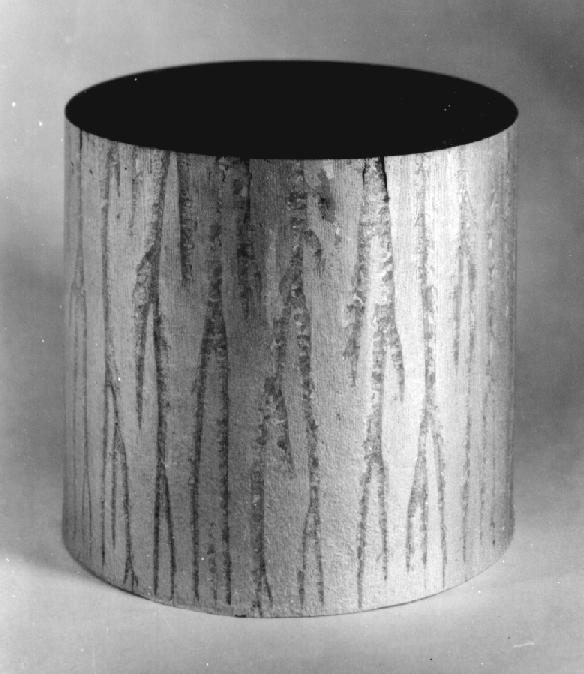
\includegraphics[height=5cm]{Chapter0/Graphics/freckle1.png}
	\caption{\$WRITE\$}
    \label{fig:freckle1}
  \end{subfigure}
   %------------
   \qquad %\hspace{2cm}
   \begin{subfigure}[t]{0.25\textwidth}
    \centering
	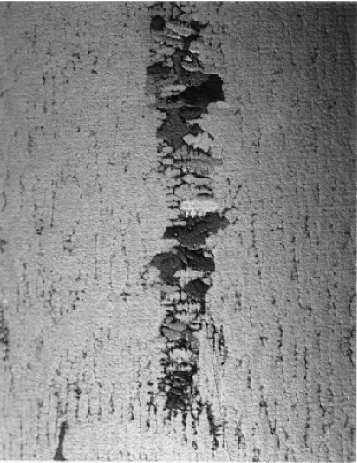
\includegraphics[height=5cm]{Chapter0/Graphics/freckle2.png}
	\caption{\$WRITE\$}
    \label{fig:freckle2}
  \end{subfigure}
   %------------
\caption{Freckles in directional casting of nickel-base superalloys} 
\label{fig:freckle}
\end{figure}
%--------------------------------------------------------
\section{Industrial Worries}
\textbf{Steel production} has continuously increased over the years to meet the industrial needs. \Cref{fig:steel_production} shows this increase between 1980 and 2013 with a 
clear dominance of the Chinese production. Quality constraints have also increased where specific grades of steel are needed in critical applications such as mega-structures
in construction and  heavy machinery. Therefore, alloys with defects are considered vulnerable and should be avoided as much as possible during the casting process. As such, steelmakers have been investing
in research, with the aim of understanding better the phenomena leading to casting problems, and improve the processes when possible.
\begin{figure}[htbp]
\centering
\begin{tikzpicture}
 \pgfkeys{%
    /pgf/number format/set thousands separator = {}}
\begin{axis}
[
	table/col sep=comma,
	smooth, %ybar
	stack plots=y,
	area style,
	enlarge x limits=false,
	legend pos=north west,
	scaled ticks=true,
	xlabel=Year,
	ylabel=Production (tons),
	xticklabel style={/pgf/number format/fixed},
	xtick={1980,1990,2000,2010},
	%x tick label style={rotate=45,anchor=east},
	%width=0.5\textwidth
]
\addplot table [x=Year, y expr=\thisrow{EU}*1000] {Chapter0/Data/steel_production.csv} \closedcycle ;
%\addlegendentry{EU (27)}
\addplot table [x=Year, y expr=\thisrow{China}*1000] {Chapter0/Data/steel_production.csv}\closedcycle;
%\addlegendentry{China}
\addplot table [x=Year, y expr=\thisrow{World}*1000] {Chapter0/Data/steel_production.csv}\closedcycle;
%\addlegendentry{World}
\legend{EU (27), China, World}
\end{axis}
%\addplot table [x expr=\coordindex, y=EU] {Chapter0/Data/steel_production.csv};
\end{tikzpicture}
\caption{Evolution curves of crude steel worldwide production from 1980 to 2013}
\label{fig:steel_production}
\end{figure}

\textbf{Simulation software} dedicated to alloy casting is one of the main research investments undertaken by steelmakers. These tools coming from academic research
are actively used to optimize the process. However, few are the tools that take into account the casting environment. For instance, the continuous casting process, in
\cref{fig:cc_process}, is a chain process where the last steps involve rolls, water sprays and other components. A dedicated software is one that can provide the
geometric requirements with suitable meshing capabilities, as well as respond to metallurgical and mechanical requirements, mainly:
\begin{itemize}
\itemsep0em
\item handling moulds and their interaction with the alloy (thermal resistances ...)
\item handling alloy filling and predicting velocity in the liquid and mushy zone
\item handling thermomechanical stresses in the solid
\item handling multicomponent alloys and predicting macrosegregation
\item handling finite solute diffusion in solid phases
\item handling real alloy properties (not just constant thermophysical/thermomechanical properties)
\end{itemize}
%-------------------------------------------------------------------------------------------------------------------------------------------------
\section{Project context and objectives}
%--------------------------------------------------------
\subsection*{Context}
The European Space Agency (ESA) has been actively committed, since its foundation in 1975, in the research field.
Its covers not only exclusive space applications, but also fundamental science like solidification. 
This thesis takes part of the ESA project entitled \ccemlcc, abbreviating
"\textbf{C}hill \textbf{C}ooling for the \textbf{E}lectro-\textbf{M}agnetic \textbf{L}evitator in relation with 
\textbf{C}ontinuous \textbf{C}asting of steel".
The three-year contract from 2011 to late 2014 denoted \ccemlcc II, was preceded by an initial project phase, \ccemlcc I,
from 2007 to 2009. The main focus is studying containerless solidification of steel under microgravity conditions. 
A chill plate is later used to extract heat from the alloy, simulating the contact effect with a mould in continuous casting
or ingot casting.
A partnership of 7 industrial and academic entities was formed in \ccemlcc II. A brief summary of each partner's commitment:\\

\textbf{Academic partners} 
 \begin{itemize}
\itemsep0em
\item CEMEF (France): numerical modelling of microgravity chill cooling experiments
\item DLR (German Aerospace Centre) and RUB university (Germany):  preparation of a chill cooling device 
for the electromagnetic levitator,  microgravity testing and investigation of growth kinetics 
in chill-cooled and undercooled steel alloys
\item University of Alberta (Canada): Impulse atomization of the D2 tool steel 
\item University of Bremen - IWT institute (Germany): study of melt solidification in atomization processing
\end{itemize}

\textbf{Industrial partners}
\begin{itemize}
\itemsep0em
\item ARCELORMITTAL (France): elaboration of a series of steel grades used in microgravity and ground studies
\item METSO Minerals Inc.  (Finland): material production with D2 tool steel for spray forming
\item TRANSVALOR (France): development and marketing of casting simulation software \thercast
\end{itemize}

CEMEF, as an academic partner, contributed to the work by proposing numerical models in view of predicting the chill cooling of steel droplets. 
A first model was developed by \citet{rivaux_simulation_2011} whereas the present discusses a new model. 
The experimental work considered various facilities and environments to set a droplet of molten alloy in levitation: 
electromagnetic levitation or EML (\cref{fig:eml}) for ground-based experiments, 
microgravity in parabolic flight or sounding rockets and last, microgravity condition on-board the International Space Station (ISS)
%---------
\begin{figureth}
% textwidth 
{0.5}
%path 
{Chapter0/Graphics/eml1.jpg}
% caption
{Electromagnetic levitation}
% label
\label{fig:eml}
\end{figureth}
%-------------------------------------------------------------------------------------------------------------------------------------------------
\subsection{Ojectives and outline}
The scope of the present thesis is macrosegregation with liquid dynamics assuming a fixed solid phase, i.e. no account of solid 
transport (e.g. equiaxed crystals sedimentation) and no account of solid deformation. In CEMEF, this framework has been the same for previous 
work by \citet{gouttebroze_modelisation_2005, liu_finite_2005, mosbah_multiple_2008, rivaux_simulation_2011, carozzani_developpement_2012}.
Nevertheless, many modelling features evolved with time such as going from two-dimensional to three-dimensional modelling, resolution scheme
for each of the conservation equations: energy, chemical species and liquid momentum, Eulerian or Lagrangian method, modelling of grain structure and others.
In this thesis, we propose a numerical model that takes into account i) the energy conservation in a temperature formulation based on a thermodynamic database mapping,
ii) the liquid momentum conservation with thermosolutal convection and solidification shrinkage as driving forces, iii) solute mass conservation and iv) solidification paths at full equilibrium for multicomponent alloys microsegregation. Moreover, all equations are formulated in a pure Eulerian context while using the Level Set method to
keep implicitly track of the interface between the alloy and surrounding gas. To my knowledge, this work combining macrosegregation prediction using the level set methodology to track the metal-air interface during shrinkage has no precedent in the literature.

\emph{Numerical tools: Cimlib relying on PETSc, parallelized with MPICH2, paraview and python as tools for postprocess and analysis. \\
The previously mentionned simulation requirements are not met in a single casting software package. Nevertheless, \thercast is a promising tool that already 
handles a part of the above points. The current thesis developments are done using C++ language as a part of the
in-house code, known as \cimlib \citep{digonnet_cimlib:_2007, mesri_advanced_2009}. 
This fully parallel library is the main academic research support for \thercast.\\ \\ }

\paragraph{Outline}
Each chapter content


%--------------------------------------------------------
\subsection*{Biblio test}
\citet{carozzani_direct_2013} is textual \\
\citep{carozzani_direct_2013} is parenthetical \\
%--------------------------------------------------------
\subsection*{Cross reference test}
ref gives \ref{eq:betaT} \\
cref gives \cref{eq:betaT} \\
Cref gives \Cref{eq:betaT} \\
autoref gives \autoref{eq:betaT} \\


ref gives \ref{fig:porosity1} \\
cref gives \cref{fig:porosity1} \\
Cref gives \Cref{fig:porosity1} \\
autoref gives \autoref{fig:porosity1} \\


%\section*{Trying \emph{SIUNITX}}
%Here i wana test the SI units package via the commands \num{.3e45} and the unit \si{\kilo\metre}
%then i wanted to see if we combine both via \SI{.3e45}{\kilo\metre} then finally my personal command
%\SI{231e-4}{\uacceleration} \\
%\SI{231e-4}{\ucomposition} C \\
%\SI{231e-4}{\uvelocity} \\
%\SI{231e-4}{\uconductivity} \\
%\SI{231e-4}{\umasscapacity} \\
%\SI{231e-4}{\uvolumecapacity} \\
%Will it work \num{.3e45}   ,  \num{3.45d-4}   , \numlist{10;30;50;70} ,  \numrange{10}{30}